\chapter{Results}
\label{chap:results}

\section{Method development}
\label{section:Results_Method_Development}
\subsection{Haemocyte medium: inhibition of aggregation}
The proportions of aggregated haemocytes in MPSS, ACB and MAS are plotted against time post-withdrawal in Fig. \ref{fig:aggregation}, together with the mean proportions predicted from the sub-models (\ref{eq:agg_submodels}a-c) of the fitted log-logistic model. The estimated model parameters 

\begin{figure}[!ht]
    \centering
    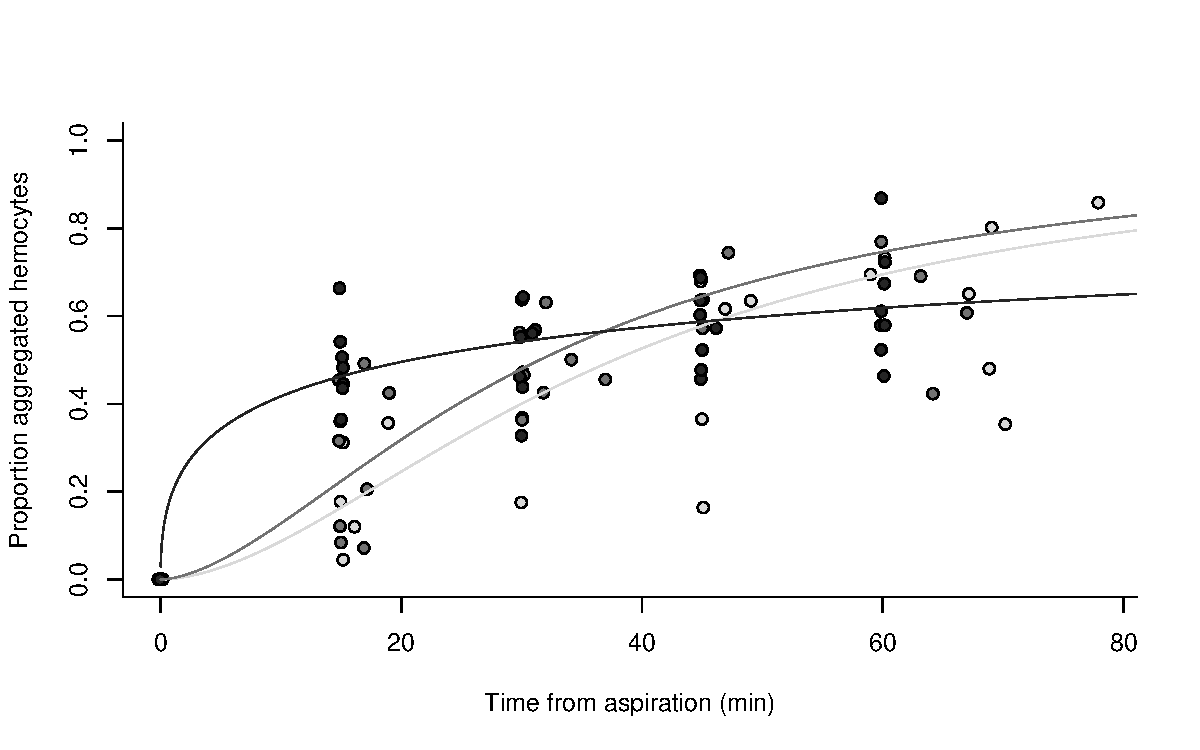
\includegraphics[width=1.0\textwidth]{figures/Method development/agg_plot_scaled.pdf}
    \caption{The proportion of aggregated hemocytes in 250 \micro L hemolymph withdrawn into an equal volume of Modified Alsever's Solution (\protect\lysegraacircle, n=7), Anticoagulant Buffer (\protect\graycircle, n=8) or Marine Physiological Saline Solution (\protect\darkgraycircle, n=8), plotted against time (min) after withdrawal from the posterior adductor muscle. The three regression lines illustrate the predicted proportions at time t for the three different buffers, as predicted by the fitted logistic regression model.}
    \label{fig:aggregation}
\end{figure}
 
\begin{subequations}
    \label{eq:agg_submodels}
    \begin{equation}
        \text{MPSS:} ~ y_{i} = \dfrac{1}{1 + e^{-(-1.3874 + 0.4573\times log(x_{i}))}} + \epsilon_i
    \end{equation}
    \begin{equation}
         \text{ACB:} ~ y_{i} = \dfrac{1}{1 + e^{-(-5.7779 + 1.6748\times log(x_{i}))}} + \epsilon_i \label{eq:ACB}
    \end{equation}
    \begin{equation}
        \text{MAS:} ~ y_{i} = \dfrac{1}{1 + e^{-(-6.4301 + 1.7719\times log(x_{i}))}} + \epsilon_i
    \end{equation}
\end{subequations}
  



Interpreting the logistic sub-models, it is evident that MAS and ACB effectively slowed the rate of aggregation during the first 30 minutes post-withdrawal. When MAS was used as hemocyte medium, the predicted mean proportion of aggregated hemocytes after 15 minutes was 0.16, 95\% CI [0.12, 0.22]. This was not significantly different from the predicted mean proportion when ACB was used (0.22, 95\% CI [0.18, 0.28]), but both buffers containing EDTA and lacking free Ca$^{2+}$ were predicted to have significantly lower hemocyte aggregation after 15 minutes, compared to samples that were withdrawn into MPSS and kept on ice (0.46, 95\% CI [0.33, 0.60]).

Although the model is over-dispersed, these estimates provided some insight into the three factor's relative abilities to prevent hemocyte aggregation within the first hour post-withdrawal. The combination of a Ca$^{2+}$-free and EDTA-containing buffer was effective in reducing hemocyte aggregation compared to simply diluting and keeping samples on ice. When using the latter method, visible aggregates were usually formed within the syringe immediately after hemolymph aspiration, even though the hemolymph saline was been pre-chilled at $\SI{4}{\celsius}$. For this method to be effective, the hemolymph most likely has to be diluted many-fold. Such an approach would be inconvenient when preparing microscopy slides of a certain desired cell density, and too time-consuming when acquiring 10.000 events on a flow cytometer. This approach was therefore ruled out of question.

Comparing the relative effectiveness of MAS and ACB in preventing hemocyte aggregation, it is evident that neither citrate or maintaining a slightly acidic pH is required for the purpose. It might be that the slightly higher concentration of EDTA in ACB compensates for the lack of citrate. But either way, the acidic pH most likely plays a minor role. Since high concentrations of EDTA has been reported to impair hemocyte viability by some authors (\cite{Grandiosa2018, Burkhard2009}), a further comparison of MAS and ACB with regards to acute effects on viability had to be investigated.

\subsection{Haemocyte medium: effect on viability}
 The percentage of necrotic hemocytes kept in at the three timepoints are presented in figure \ref{fig:BufferViability}. \lipsum[2]

\begin{figure}[!ht]
    \centering
    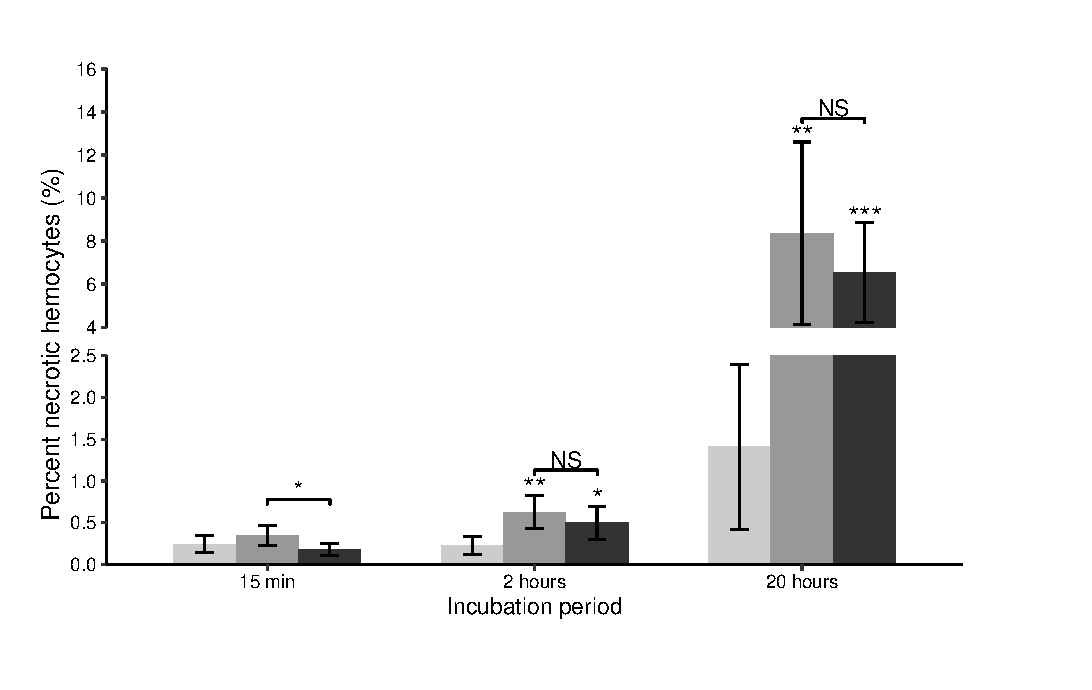
\includegraphics[width=1.13\textwidth]{figures/Method development/grouped bargraph scaled.pdf}
    \caption{The mean percentages of TO-PRO$^{TM}$-3 Iodide positive hemocytes after 15 minute, 2 hours and 20 hours incubation in \protect\lysegraabox \ Marine Physiological Saline Solution (n=8), \protect\customgraybox \ Anticoagulant Buffer (n=8) or \protect\darkgraybox \ Modified Alsever's Solution (n=8). Calcein acetoxymethyl (Invitrogen$^{TM}$) was used as a live cell counter-stain. Each datapoint is expressed as a percentage of 10.000 recorded hemocyte events, and the error bars represent 95\% confidence intervals of group means. Asterisks above error bars represent significance level of two sample t-test comparisons with }
    \label{fig:BufferViability}
\end{figure}

- Report results fro where I checked if EDTA changed the cytogram, because it would be nice to report that it doesn't affect them during the 15 minute incubation period.

\subsection{Cytologic characterization of \emph{M. edulis} hemocyte subpopulations}
\label{subsection:Results_cytchar}
The hemolymph of \emph{Mytilus edulis} comprised a mixed population of cells differing in size, granularity, morphometrics and Wright's-Giemsa staining profiles. If the haemocytes were allowed to spread prior to fixation and staining, the diversity further expanded as cells took on a variety of shapes and/or developed cytoplasmic extensions. From these morphological criteria, a total of three distinct cell types could be identified by light microscopy.

Based on the basophilic or eosinophilic nature of their granules and other cytoplasmic contents, cytologic staining with 3 \% Wright's-Giemsa or the Hemacolor\textsuperscript{\textregistered} kit gave rise to two distinct staining profiles: basophilic and eosinophilic haemocytes. The cytoplasm of eosinophilic hemocytes (Figure \ref{fig:celltypes}, K-O) were densely packed with pink to dark purple granules of varying size and abundance. Hence, they are referred to as eosinophilic granulocytes herein. Their individual granules were usually not distinguishable in a non-spread state, but instead gave their cytoplasm an irregular pink color (Figure \ref{fig:celltypes}, K and O). These haemocytes had cell diameters in the range of 6-16 \micro m, with a mean of 9.06$\pm1.25$ \micro m. Two strikingly homogeneous features of this cell type was a small acentrically located nucleus, and a regular spherical outline in a non-spread state. With abundant pink cytoplasm making up the majority of the cells' surface area - even in the smallest specimens - the eosinophilic granulocytes could also be characterized by a low nuclear-cytoplasmic ratio (N:C ratio). If not fixed and stained before smearing - or within minutes of applying haemolymph to a glass slide - eosinophilic granulocytes were almost exclusively observed as spread cells. 

\begin{figure}[!ht]
    \centering
    \includegraphics[width=1.0\textwidth]{figures/Anatomy/cell types brightfield updated 2.pdf}
    \caption{100$\times$ brightfield micrographs of the three haemocyte types found in the haemolymph of \emph{Mytilus edulis}, fixed and stained on glass slides with the Hemacolor\textsuperscript{\textregistered} kit before the hemocytes had time to spread notably. \textbf{(A-E)} Blast-like hyaline basophils. \textbf{(F-J)} Basophilic granulocytes. \textbf{(K-O)} Eosinophilic granulocytes. Samples were withdrawn into MPSS (1:1), scale bars = 10 \micro m.}
    \label{fig:celltypes}
\end{figure}

Compared to the eosinophilic granulocytes, the basophilic hemocytes encompassed a more heterogeneous population. Common to all of them were a larger nucleus that occupied more of the cells' total surface area (higher N:C ratio). The shape of which varied from spherical to oval, or had a distinct bean-shaped or irregular outline. But judged from the morphological criteria of cell size, granularity and N:C ratio, there were essentially two distinct subpopulations of basophilic haemocytes. One population of small hyaline blast-like haemocytes (5.63 $\pm{0.72}$ \micro m) displaying only a marginal rim of dove blue cytoplasm and no apparent cytoplasmic granules (Figure \ref{fig:celltypes}, A-E), and one population of larger haemocytes (8.07 $\pm{1.25}$ \micro m), displaying abundant basophilic cytoplasm with varying degrees of cytoplasmic granulation and vacuolation (Figure \ref{fig:celltypes}, F-J). The basophillic granules appeared much smaller than those of the eosinophilic granulocytes, and were usually not very conspicuous unless haemocytes were subjected to osmotic swelling prior to fixation and staining. Under differential interference contrast (DIC) illumination however, their granules created highly irregular surface topographies in spread cells that could be observed without such treatment. On the basis of these morphological differences, the basophilic haemocytes were subdivided into blast-like haemocytes and basophilic granulocytes herein. 

\begin{figure}[!ht]
    \centering
    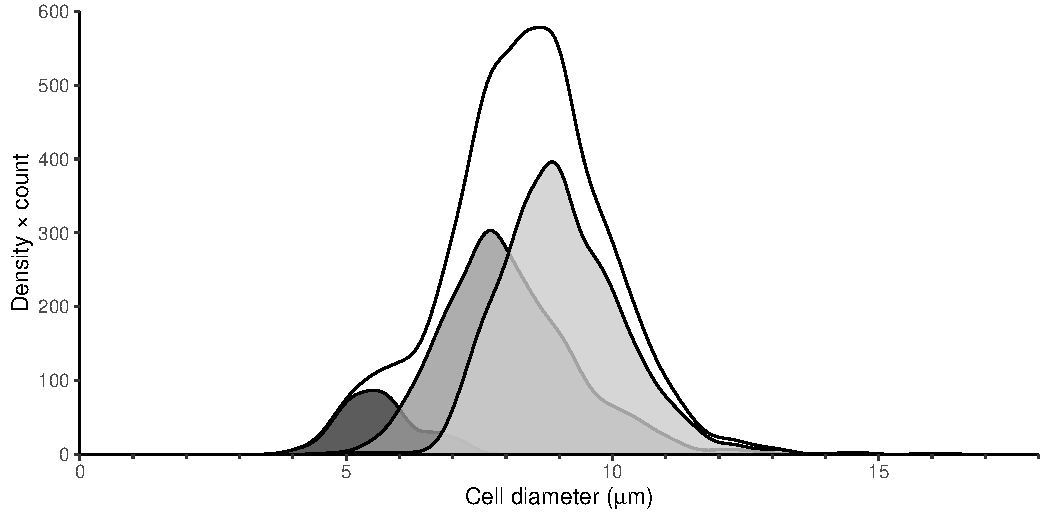
\includegraphics[width=1.0\textwidth]{figures/Anatomy/diameters scaled density plot.pdf}
    \caption{Size distribution of \protect\dimgraybox \ small blast-like basophils (n=154), \protect\lightgraybox \ basophilic granulocytes (n=821), \protect\lysegraabox \ eosinophilic granulocytes (n=1030) and \protect\whitebox \ the total haemocyte population of \emph{Mytilus edulis} (n=2005). The diameters of 100 formaldehyde-fixed haemocytes was measured in each of 20 individual mussels, and the density was scaled to the number of observations of each cell type.}
    \label{fig:Diameters}
\end{figure}

The size distributions of the three haemocyte types are shown as three kernel-smoothened density plots in Figure \ref{fig:Diameters}, together with that of the total haemocyte population. The densities have been scaled to the number of observations of each cell type, such that their relative proportions can be visualized. In the 20 adult mussels examined here, the small blast-like basophils were the least abundant cell type, making up 7.9 $\pm{5.6}$ \% of the total haemocyte population. In 14 out of 20 mussels, the blast-like basophils were followed by the basophilic granulocytes, with a mean relative proportion of 40.7 $\pm{12.9}$ \%. In spite of constituting similar proportions as the basophilic granulocytes in several mussels, the eosinophilic granulocytes were the most abundant cell type in the haemolymph of \emph{M. edulis}, constituting 51.5 $\pm{15.3}$ \% of the total haemocyte population, on average. The relative proportions of basophilic and eosinophilic granulocytes did however vary to a large extent between individual mussels, as reflected by their standard deviations. [Should I include t.tests in this section? - note: unequal sample sizes]

When incorporating the Coulter Counter data in this section, this article can be used to reference the accuracy of the electronic cell size method which it uses: Mattern CFT, Brackett FS, Olson BJ. Determination of number and size of particles by electrical gating: blood cells. J Appl Physiol 1957;10:56–70


\subsection{Flow cytometric characterization of haemocyte subpopulations by light-scatter}
\label{subsection:Results_FlowChar}
A maximum of three distinct subpopulations could be separated according to Forwards scatter (FCS) vs. Side scatter (SSC) in suspensions of living haemocytes. These subpopulations correspond to clusters 1, 2 and 3 in Fig. \ref{fig:fsc_vs_ssc}, where the haemocytes of three representative mussels have been displayed with SSC on logarithmic and linear scales. The adjunct histograms in Fig. \ref{fig:fsc_vs_ssc}A clearly illustrates that the three clusters of events are separated according to SSC, while cluster 2 and 3 are substantially overlapping with regard to FSC.

\begin{figure}[!ht]
    \centering
    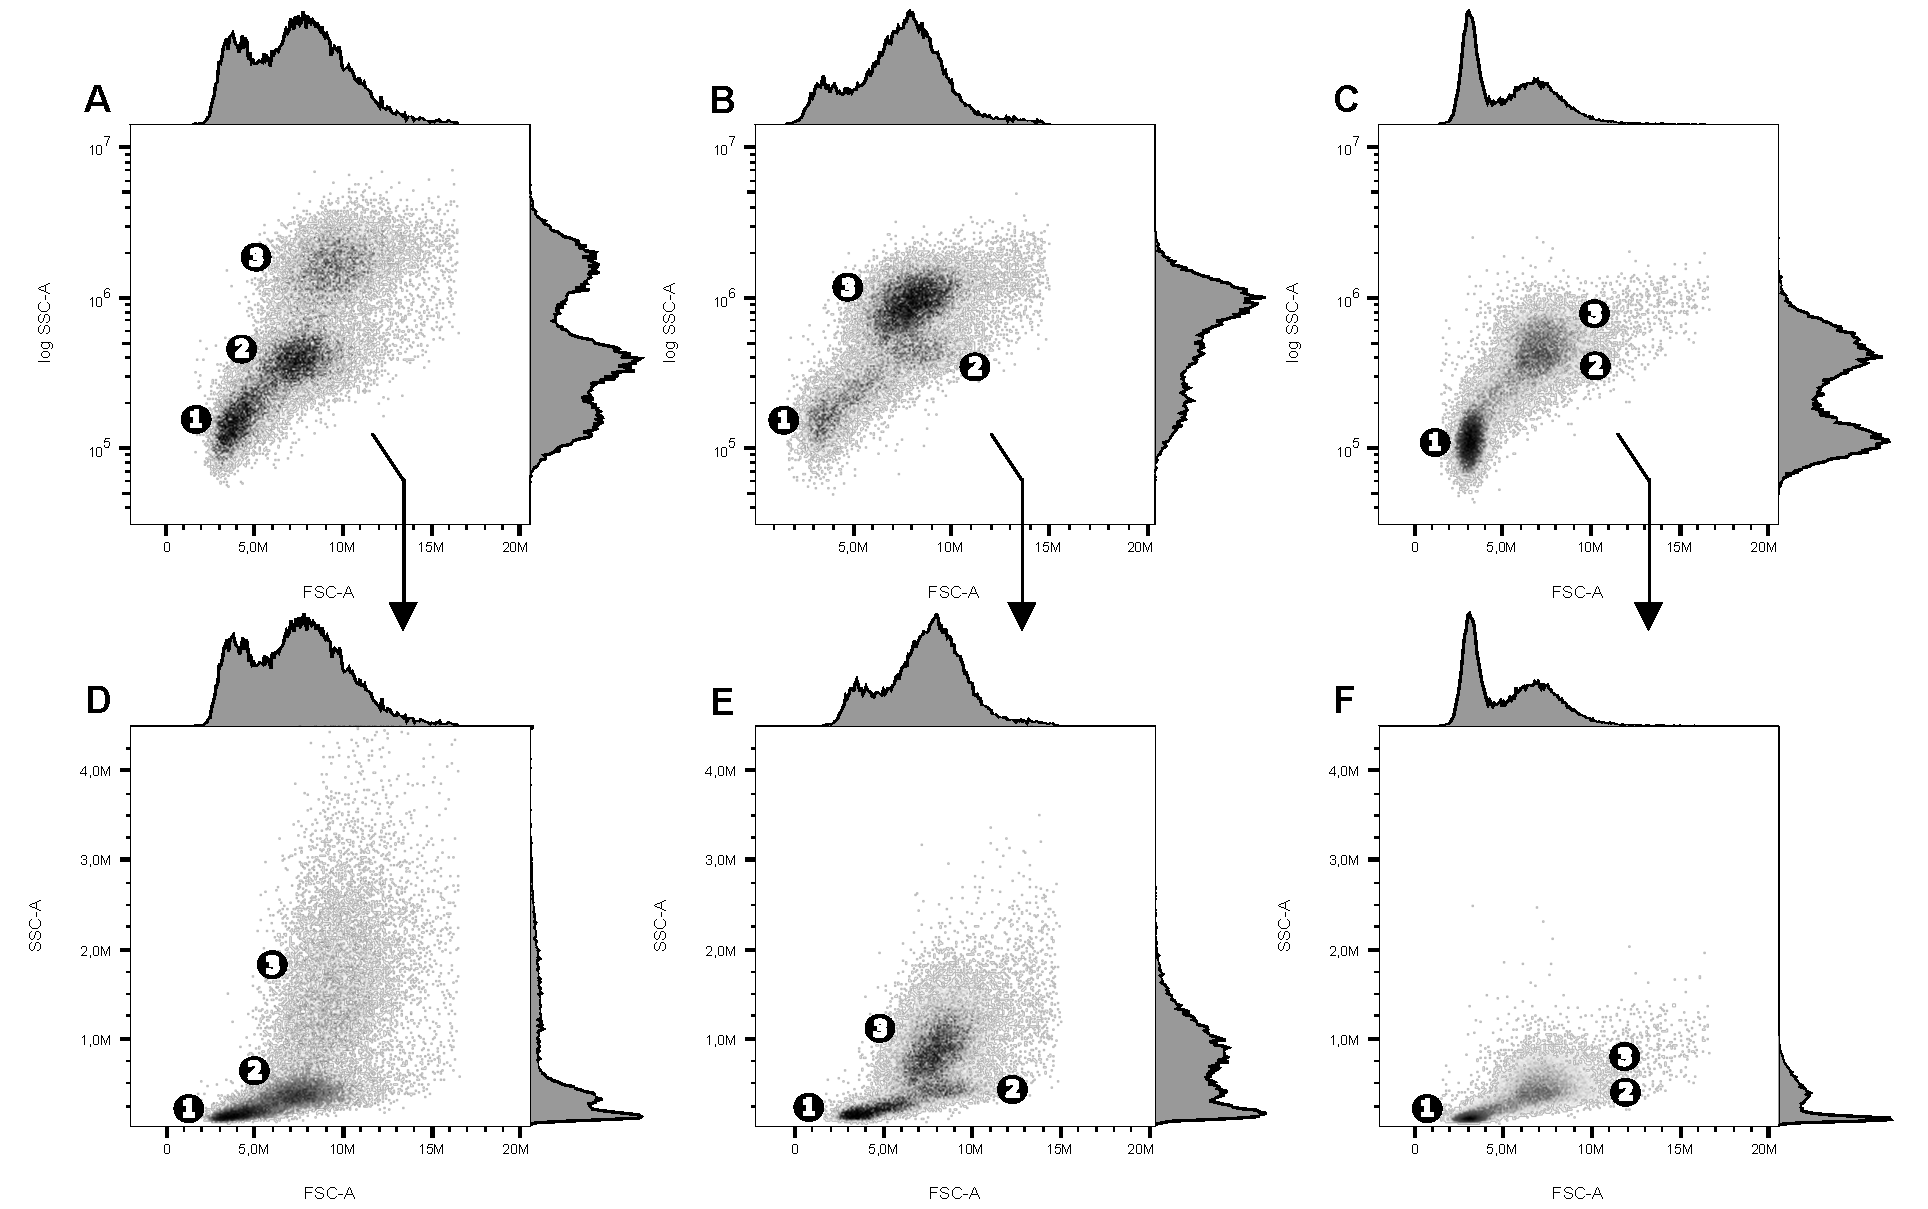
\includegraphics[width=1.0\textwidth]{figures/Gating strategy/scatter profiles 30k with let num.pdf}
    \caption{\textbf{Hemocyte subpopulations distinguishable according to FSC and SSC. measurements with the BD Accuri C6 Plus Benchtop Flow Cytometer.} The light-scatter profiles of three representative adult mussels are displayed with SSC on logarithmic \textbf{(A-C)} and linear \textbf{(D-F)} scales to illustrate the observed variation in the degree of separation between cluster 2 and 3. Adjunct histograms were included to underline the degree of separation from the individual parameters.}
    \label{fig:fsc_vs_ssc}
\end{figure}

Describe cluster 1, 2 and 3 in terms of relative SSC and FSC, and suggest which cell types they represents based on size and granularity:

The events populating cluster 1 exhibited low FSC- and SSC-values relative to cluster 2 and 3, suggesting that it is populated by small and uncomplex cells. Events in both clusters 2 and 3 display higher FSC-values, but are often only partially separated according to SSC.

and are most likely corresponding to the small agranular cells shown in Figure [ref to Figure with cell morphology and Giemsa staining profile], with a large oval nucleus and a thin rim of basophilic staining cytoplasm. Herein we will refer to them as agranular basophils according to their Giemsa staining profile. Because of their smaller size relative to the cells in cluster 2 and 3; they are readily distinguishable with a separate peak in Coulter Counter particle-size distributions, and have cell diameters between 5.5-8 \micro m [include Figure].

\subsection{Relating the cytologically defined cell types to light-scatter profiles}
Hemocyte subpopulations and clusters. Light-scattering properties (optical characteristics).
The first round of Percoll separation yielded 96.1 \% eosinophilic granulocytes in the 43/90\% fraction.
The second round of percoll gradient separation yielded: 15\%-33\% interface: FCM = 97\% basophils, microscopy = 96.14 \% basophils (7.72\% blast-like and 88.42\%) (= 3.86 \% eosinophils) 43\%-90\% interface: FCM = 94\%, microscopy = 97.52 \%.

\begin{figure}[!ht]
    \centering
    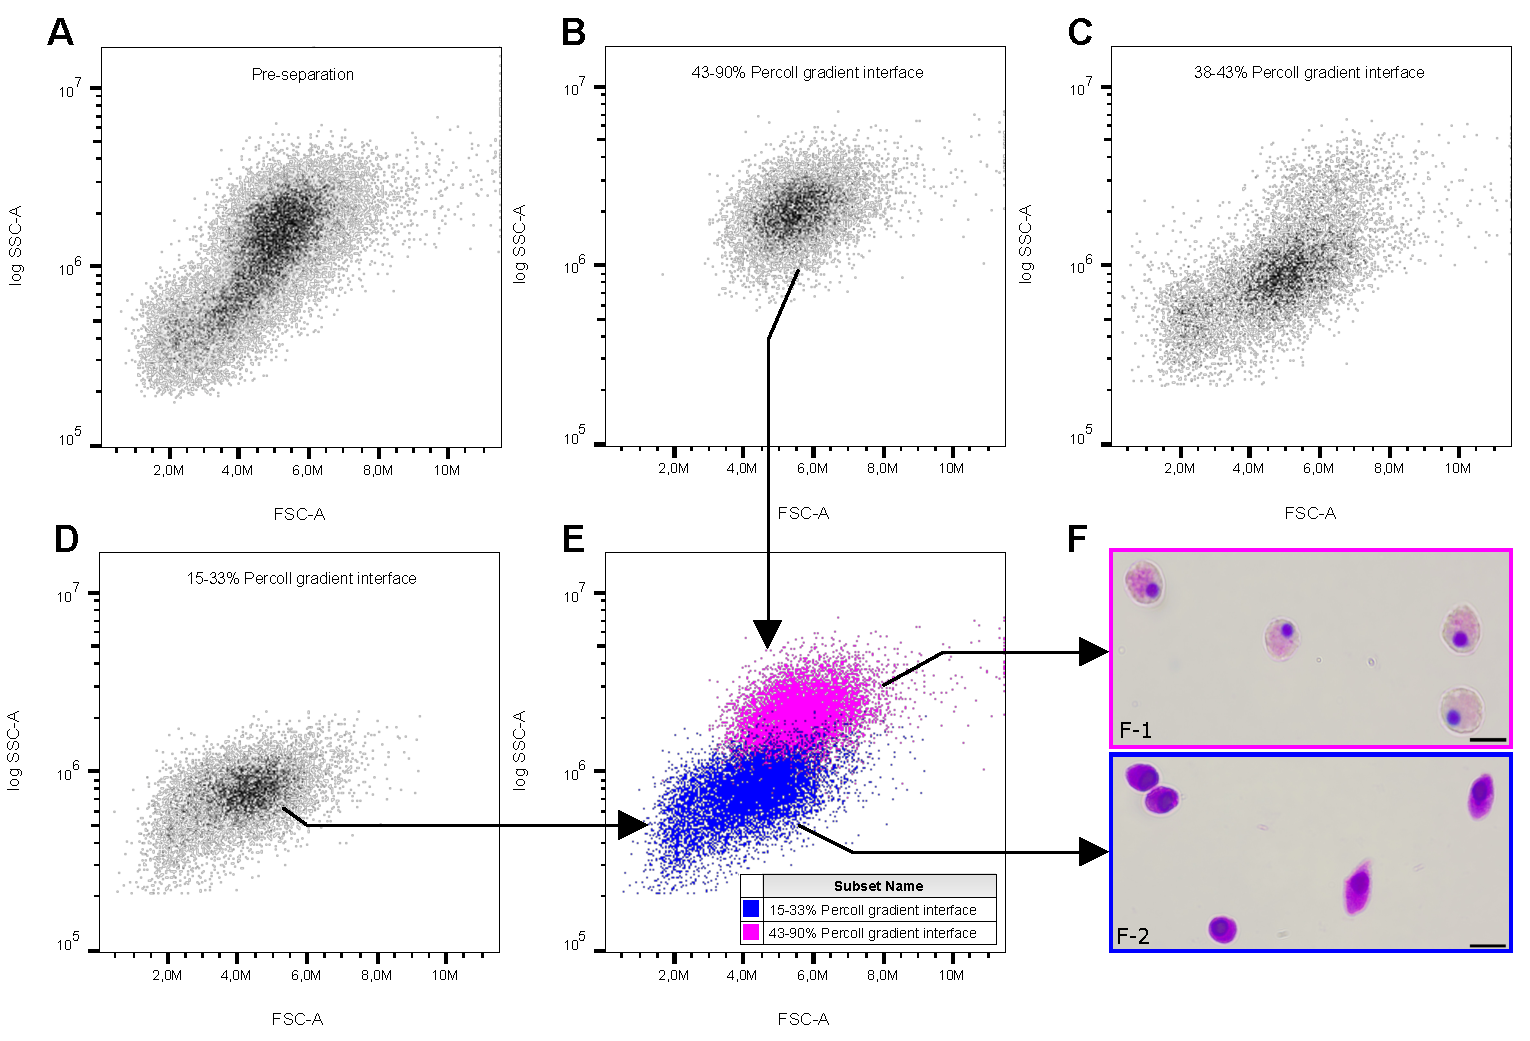
\includegraphics[width=1.0\textwidth]{figures/Method development/PERCOLL SEP II final.pdf}
    \caption{\textbf{Confirmation of the light scattering profiles of eosinophilic and basophilic granulocytes pre-separated by discontinuous density centrifugation. A} Light scattering profile of the 95\% pure eosinophilic fraction that separated out on top of the 43-90\% Percoll gradient interface. \textbf{B} Bla bla bla eosin separation bla bla...}
    \label{fig:Percoll-dotplots}
\end{figure}



\begin{figure}[!ht]
    \centering
    \includegraphics[width=1.0\textwidth]{figures/Method development/Eosin fluorescence figure.pdf}
    \caption{\textbf{Eosinophilic granulocytes can be distinguished from the two basophilic cell types according to eosin fluorescence ($\geq$ 515 nm).} Formaldehyde-fixed haemocytes stained in 0.75\% eosin and 3\% Giemsa were imaged at $\times$60 under \textbf{A)} brightfield illumination and \textbf{B)} by epifluorescence microscopy with a B-2A filter cube. The slide was mounted with Eukitt\textsuperscript{\textregistered} and coverslipped prior to microscopy. Eo: eosinophilic granulocyte; B: basophilic haemocyte; scale bars = 10 \micro m. }
    \label{fig:eosin_fluorescence_B2A}
\end{figure}



\begin{figure}[!ht]
    \centering
    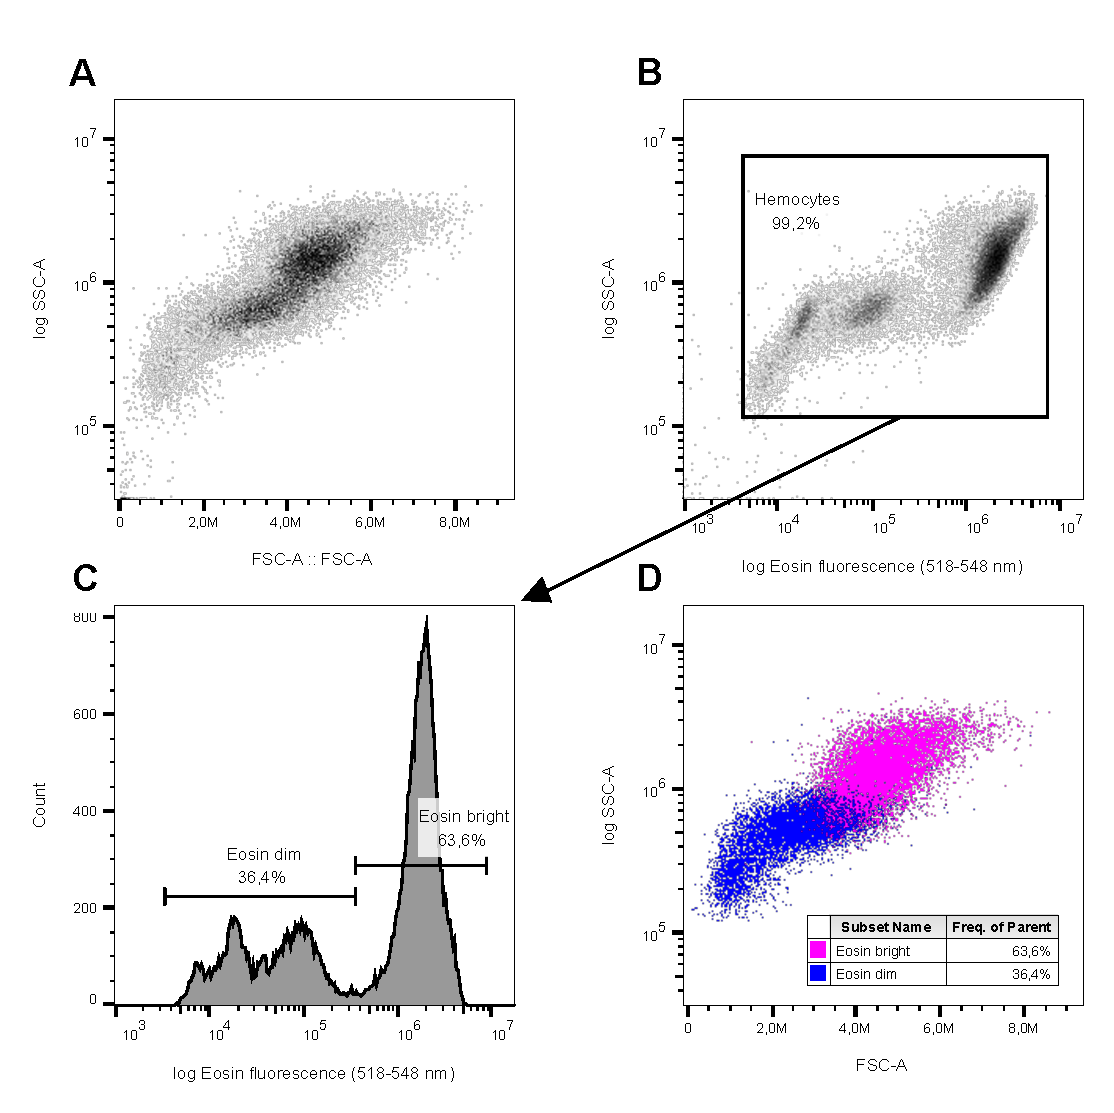
\includegraphics[width=.73\textwidth]{figures/Method development/Eosin exp figure for LaTeX.pdf}
    \caption{\textbf{Identification eosinophilic granulocytes. A)} Representative light scatter profiles of... \textbf{B)} }
    \label{fig:eosin_exp2}
\end{figure}

[After the eosinophils had sedimented in the MAS buffer (sample M2 in sedimentation dataset) for 2 hours post-withdrawal (1:1), the percentage of eosinophils remaining in suspension were 72/1075 = 6.6976 \%. The 10k ToPro3 Calcein stained plot shows 7.91\%.]
\newpage

In some adult mussels, however, the basophilic and eosinophilic granulocyte subpopulations are partly overlapping with regard to internal complexity, i.e., SSC. Since the BD Accuri C6 Plus isn't equipped with adjustable laser gain settings, these subpopulations could not be separated further instrumentally. Thus, any attempts to gate on these subpopulations based solely on light scattering profiles, would in some mussels introduce considerable uncertainty into their relative proportions. [Find the proportion of mussels where they are not well separated, and report that number instead of saying "some" mussels here.]



\subsection{Scoring of necrotic haemocytes by flow cytometry}
\subsubsection{Determination of optimal TO-PRO$^{TM}$-3 Iodide staining concentration}
Viable and \ce{MeOH}-killed haemocytes could be separated according to TO-PRO-3 Iodide fluorescence in the whole range of tested concentrations (30 nM - 8 \micro M). As shown in Fig. \ref{fig:ToPro3_stain_opt}B, the resolution between ToPro3$^{-}$ and ToPro3$^{+}$ events increased with the TO-PRO$^{TM}$-3 Iodide concentration according to the log-logistic function shown in (\ref{eq:fitted.LL4}), with a marked stagnation > 1.2 \micro M. The model explained almost all the variation in the dataset (Pseudo-R$^{2}$ = 0.99, see table \ref{tb:loglogistic_ToPro3}), and should therefore be a good predictor of the expected resolution between necrotic and viable haemocytes in the tested range of TO-PRO$^{TM}$-3 Iodide.

\begin{equation}
\label{eq:fitted.LL4}
y_{i} = \dfrac{9890700}{1 + (x_i / 0.41655)^{-0.94088}} + \epsilon_i
\end{equation}

The predicted difference in MFI at 1.2 \micro M was 7.220.000 (arbitrary units), 95\% PI[6.170.000, 8.260.000]. Since the slope of function \ref{eq:fitted.LL4} decreased rapidly for x > 0.6, the predicted difference in MFI at x = 1.2 \micro M was contained within the prediction intervals for the rest of the function's range. Furthermore, the MFI of the ToPro3$^{-}$ populations increased abruptly at concentrations $\geq$ 2 \micro M (see Table \ref{tb:ToPro3_stainopt}), indicating a potential cytotoxic effect of either TO-PRO$^{TM}$-3 Iodide or the DMSO solvent at high concentrations.

\begin{figure}[h]
    \centering
    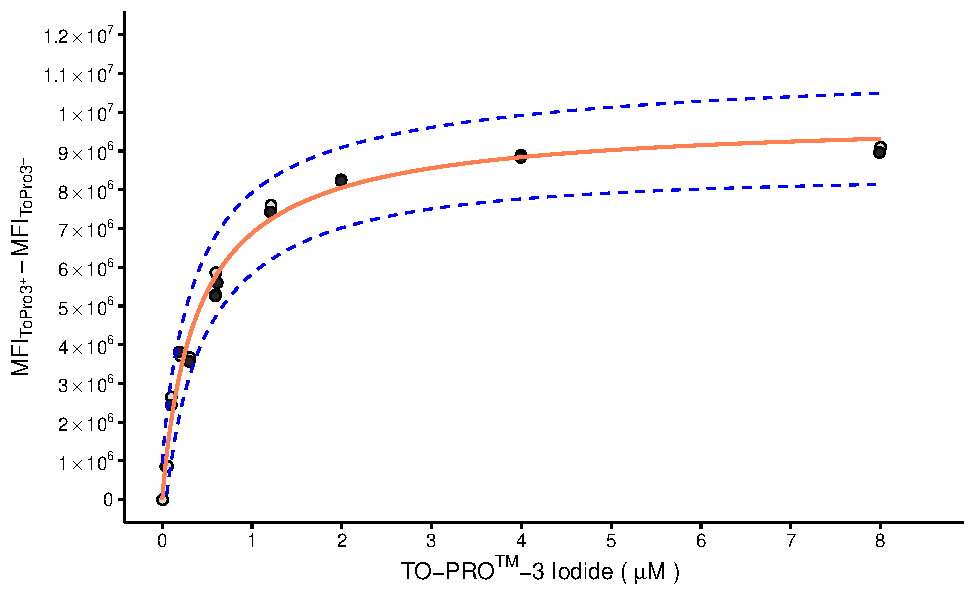
\includegraphics[width=1.0\textwidth]{figures/Method development/ToPro3 LL4.pdf}
    \caption{\textbf{Experimental determination of the optimal TO-PRO$^{TM}$-3 Iodide concentration for a dye exclusion test of membrane integrity}. 10 aliquots of pooled methanol-killed (70\% \ce{MeOH}, 30 min) and viable haemocytes (1:1) were stained with different concentrations of TO-PRO$^{TM}$-3 Iodide (30 nM - 8 \micro M). 640 nm-exited fluorescence from dsDNA-bound TO-PRO$^{TM}$-3 Iodide were collected on the FL4 detector (675/25 nm) of the BD Accuri C6 Plus flow cytometer, recording 10.000 events from each sample after 15 and 30 minute incubation. \textbf{A)} ToPro3$^{-}$ and ToPro3$^{+}$ events were gated on log scale for each sample, \textbf{B)} and their difference in mean fluorescent intensity (MFI) after 15 (\protect\lysegraacircle) and 30 minutes (\protect\darkgraycircle) of incubation were plotted against the concentration of TO-PRO$^{TM}$-3 Iodide. Red line: fitted log-logistic regression model; blue dashed lines: prediction intervals.}
    \label{fig:ToPro3_stain_opt}
\end{figure}

Taken together, these results suggested that the potential gain from increasing the staining concentration above 1.2 \micro M was limited, and not completely free of risk. The resolution between viable and necrotic haemocytes was for all practical purposes sufficient the range of 300 nm - 1.2 \micro M, but the resolution at 1.2 \micro M would simplify gating on a logarithmic scale. 1.2 \micro M TO-PRO$^{TM}$-3 Iodide was therefore preferred for scoring necrotic haemocytes by flow cytometry, together with 50 nM Calcein AM.

The results were also unambiguous regarding the incubation period. According to Figure \ref{fig:ToPro3_stain_opt}B, the resolution between viable and necrotic cells did not increase after the initial 15 minute incubation period. The MFI of necrotic haemocytes did increase somewhat in the extended incubation period, but the resolution remained unchanged due to a concurrent proportional increase among the viable haemocytes (see table \ref{tb:ToPro3_stainopt}, Appendix B). Extending the incubation period beyond 15 minutes would therefore be of little use.

\subsubsection{Method validation}
Simple linear regression was used to examine the correlation between results obtained by epifluorescent microscopy and the flow cytometric gating strategy presented in section \ref{subsubsection: gating validation}. It was found that the established quadrant gating strategy significantly predicted the the percentage of ToPro3$^{+}$ haemocytes (\%) in samples scored by epifluorescent microscopy ($\beta$ = 0.98818, t(8) = 32.8, p<.001). The data is presented in Fig. \ref{fig:method_val_1}, together with the fitted linear regression model (R$^{2}$ = 0.99, F(1, 8) = 1059, p<.001).

\begin{figure}[h]
    \centering
    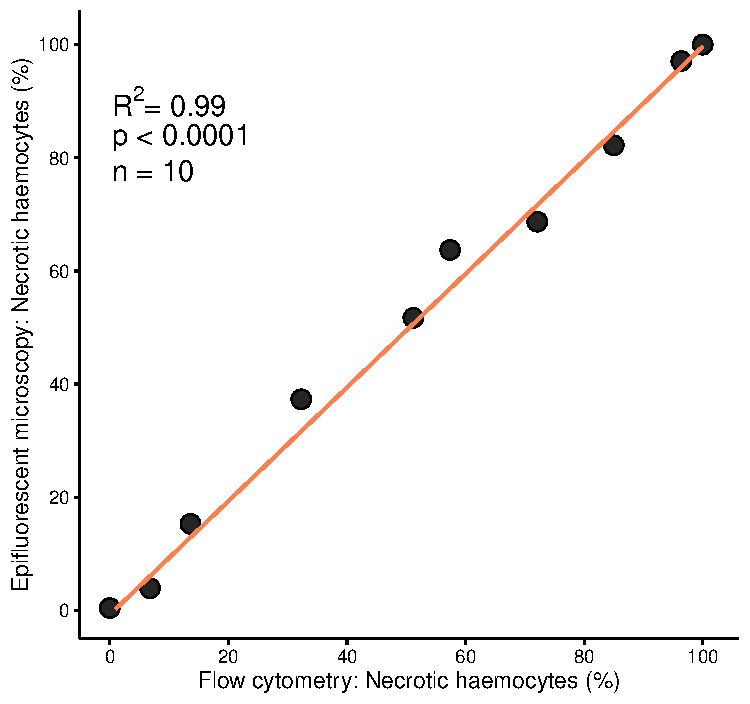
\includegraphics[width=.65\textwidth]{figures/Method development/FCM FM lin reg.pdf}
    \caption{\textbf{Correlation between necrotic haemocyte percentages scored by flow cytometry and epifluorescent microscopy.} 10 samples of freshly withdrawn haemocytes (ACB, 1:1) were mixed with methanol-killed haemocytes in semi-random proportions (0-100\%), stained with Calcein AM (50 nM) and TO-PRO$^{TM}$-3 Iodide (1.2 \micro M) and the percentage of necrotic haemocytes (\%) were scored by both flow cytometry and epifluorescent microscopy. Each datapoint represents one scored sample. Red line: fitted linear regression model.}
    \label{fig:method_val_1}
\end{figure}



\newpage
\section{Hybrid FCM/Microscopy MN Cytome Assay: Results}
\subsection{MN and other nuclear anomalies}
\subsection{Haemocyte viability: membrane integrity}
\subsection{Apoptosis assay}
\subsection{Haemocyte differential counts and concentration}

